\begin{figure}[H]
	\centering
	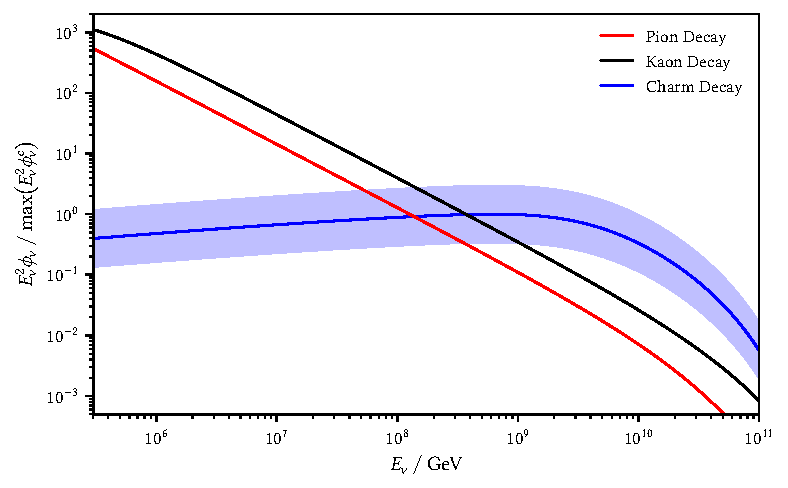
\includegraphics{../plots/build/nucleus_neutrino_spectrum.pdf}
	\caption[AGN accretion disk $\nu \kern+0.5pt$ fluence compared to $c$ decay.]
			{Expected neutrino fluence normalized to the maximum charmed hadron contribution from an AGN accretion disk.
			 Differences between the shapes of pion and kaon components compared to charm decays result from the chosen
			 view, as the flat increase observed for charmed hadrons occurs at lower energies in the case of pions and kaons
			 due to their much longer lifetimes. These decay times are listed in Sections \ref{sub:scattering} and \ref{sub:charm}
			 with Figure \ref{fig:nucleus-charm-comparison} providing the reasoning for the effects of cooling. Charmed hadrons dominate
			 the fluence from $E_\nu = \kern-0.5pt \qty{e9}{\giga\electronvolt}$ and above, lining up with prior expectations. This
			 threshold is sensitive to varying densities, with lower values producing a shift towards higher energies. A hard cutoff
			 is enforced by $E_p = \kern-0.5pt \qty{e12}{\giga\electronvolt}$ as the maximum proton energy. The same shaded uncertainty
			 band as in Figure \ref{fig:magnetar-flux-with} for charm decays as well as the scaling by $E_\nu^2$ from
			 Figure \ref{fig:magnetar-fluence-with} are adopted.}
	\label{fig:nucleus-fluence}
\end{figure}
